\documentclass[tikz]{standalone}
\usepackage{mwe,bm}
\usepackage{wrapfig}

\usepackage{stackengine}
\usetikzlibrary{tikzmark,fit,backgrounds,mindmap,decorations.text,shapes.callouts,arrows}
 \usetikzlibrary {shapes.geometric} 
\usetikzlibrary{shapes.geometric,decorations.pathmorphing,decorations.pathreplacing}
 
\renewcommand\familydefault\sfdefault
\tikzset{%
	team/.cd,
	image/.store in=\imagefile, name/.store in=\imagenamed,
	member 1/.style={image=example-image, name=A},
	member 2/.style={image=example-image, name=B},
	member 3/.style={image=example-image, name=C},
	member 4/.style={image=example-image, name=D},
	member 5/.style={image=example-image, name=E},
	member 6/.style={image=example-image, name=\textcolor{magenta}{F}},
	member 7/.style={image=example-image, name=G},
	/tikz/pics/team member/.style={code={
	\tikzset{team/.cd, member #1/.try}%
	\draw [very thick,draw=cyan, path picture={%
	\node at (path picture bounding box.center) 
{\includegraphics[width=0.6\linewidth]{\imagefile}};}]
			circle [radius=0.5];%outer circle radius
	\node [below, font=\sffamily\tiny\bfseries, text width=6em, align=center, circle, decorate, decoration={text along path}] at (0,0.5) {\imagenamed};
%\path [decorate, decoration={text along path, text={\imagenamed}, text align=center, reverse path, raise=-2pt}, font=\tiny](0,0.6) arc (90:-270:0.6cm);
	}}
}
\begin{document}
	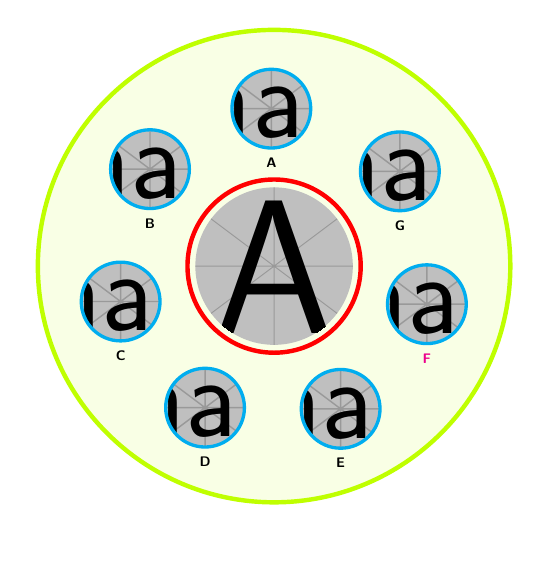
\begin{tikzpicture}
	\begin{scope}
		\draw[ultra thick, draw=lime, fill=lime!10] (0,0.0) circle (3.0cm);
		\foreach \i in {1,...,7}
		\pic at (\i*51+40:2) {team member=\i};
		\draw[ultra thick, draw=red] (0,0.0) circle (1.1cm);% red circle
		\clip (0,0.0) circle (1.0cm); %inner circle radius
		\node at (0,0.0)  {\includegraphics[width=0.4\linewidth]{example-image-a}};
	\end{scope}
\end{tikzpicture}

\end{document}